\documentclass{sbrt2017port}
%\documentclass[letterpaper, 10 pt, conference]{ieeeconf}  % Comment this line out
%\usepackage[T1]{fontenc}
%\usepackage[utf8]{inputenc}
%\usepackage[latin1]{inputenc}
%\usepackage{graphicx}
%\usepackage{gensymb}
%\usepackage{textcomp}
%\documentclass[a4paper, 10pt, conference]{ieeeconf}
\usepackage{gensymb}
\usepackage{graphicx}
\usepackage{cite}
\usepackage{amsmath}
\usepackage{fixmath}
\usepackage[none]{hyphenat}
\usepackage{textcomp}
\usepackage{url}
\sloppy

\setlength{\textfloatsep}{1pt}

\setlength{\voffset}{-0.5in}
\setlength{\textheight}{737pt}
%\setlength{\textwidth}{430pt}
%\IEEEoverridecommandlockouts

%\overrideIEEEmargins

\begin{document}

\title{Estimação de Ângulo de Chegada de Sinais de Áudio por Método Não Paramétrico Clássico}

%\author{João e Maria
%\thanks{João e Maria¸
%Departamento de Engenharia de Comunicações, Universidade Federal do Rio Grande do Norte, Natal-RN, Brasil, E-mails: vicente.gppcom@gmail.com.} }

\author{Carlos A. de Lima Filho, Matheus F. de S. Dória, Danilo de S. Pena, Allan de M. Martins, Vicente A. de Sousa Jr.
\thanks{Os autores Carlos A. de Lima Filho, Matheus F. de S. Dória e Vicente A. de Sousa Jr. são do
 Departamento de Engenharia de Comunicações (DCO), da Universidade Federal do Rio Grande do Norte (UFRN), Natal-RN, Brasil, e-mails: carlos.gppcom@gmail.com, matheusf.gppcom@gmail.com, vicente.gppcom@gmail.com. O autor Allan de M. Martins pertence ao Departamento de Engenharia de Computação e Automação (DCA), da UFRN, e-mail: allan@dca.ufrn.br. Os autores Danilo de S. Pena (danilo.gppcom@gmail.com), Allan de M. Martins e Vicente A. de Sousa Jr. pertencem ao Programa de Pós-Graduação em Engenharia Elétrica e de Computação (PPgEEC), da UFRN.}}

\maketitle

\markboth{XXXVI SIMPÓSIO BRASILEIRO DE TELECOMUNICAÇÕES E PROCESSAMENTO DE SINAIS - SBrT2018, 16-19 DE SETEMBRO DE 2018, CAMPINA GRANDE, PB} {XXXVI SIMPÓSIO BRASILEIRO DE TELECOMUNICAÇÕES E PROCESSAMENTO DE SINAIS - SBrT2018, 16-19 DE SETEMBRO DE 2018, CAMPINA GRANDE, PB}

%\begin{document}
%\maketitle
%\thispagestyle{empty}
%\pagestyle{empty}

%%%%%%%%%%%%%%%%%%%%%%%%%%%%%%%%%%%%%%%%%%%%%%%%%%%%%%%%%%%%%%%%%%%%%
%%%%%%%%%%%%%%%%%%%%%%%%% ABSTRACT %%%%%%%%%%%%%%%%%%%%%%%%%%%%%%%%%%
%%%%%%%%%%%%%%%%%%%%%%%%%%%%%%%%%%%%%%%%%%%%%%%%%%%%%%%%%%%%%%%%%%%%%

\begin{resumo}
Este artigo apresenta a avaliação de desempenho de um método não paramétrico clássico para estimação de ângulo de chegada para ondas acústicas. Por meio do periodograma é estimado a densidade espectral, que determina a frequência dominante da fonte. Posteriormente, essa informação é utilizada para determinar o ângulo de chegada do sinal recebido. O desempenho do método foi analisado e comparado para dados sintéticos e reais, obtidos a partir de um \textit{setup} de medição próprio. Os resultados de validação com sinais sintéticos indicam, como esperado, um comportamento decrescente do erro médio quadrático da estimação do ângulo ao se aumentar a SNR do sinal recebido. Já para os dados experimentais, o desempenho satisfatório do método de estimação advoga a favor de sua utilização para validação de medições reais.
\end{resumo}

\begin{chave}
Ângulo de chegada, Estimação não-paramétrica, Periodograma, Acústica.
\end{chave}

\begin{abstract}
This paper presents a performance evaluation of a classical non-parametric method for angle of arrival estimation for acoustic waves. The Periodogram technique is used in order to estimate the power spectral density, which determines the dominant frequency of the source. With this information, the angle of arrival of the received signal is determinated. The performance of the method is analyzed and compared using simulated data, and real data obtained from a own measurement setup. The validation results with simulated signals indicate, as expected, a decreasing behavior of the mean square error of angle estimation when increasing the SNR of received signal. As for the experimental data, the satisfactory performance of the estimation method claims its use for the validation of real measurements.
\end{abstract}

\begin{keywords}
Angle of arrival, Non-parametric estimation, Periodogram, Acoustics.
\end{keywords}


%%%%%%%%%%%%%%%%%%%%%%%%%%%%%%%%%%%%%%%%%%%%%%%%%%%%%%%%%%%%%%%%%%%%%
%%%%%%%%%%%%%%%%%%%%%%%%% INTRODUÇÃO %%%%%%%%%%%%%%%%%%%%%%%%%%%%%%%%
%%%%%%%%%%%%%%%%%%%%%%%%%%%%%%%%%%%%%%%%%%%%%%%%%%%%%%%%%%%%%%%%%%%%%

\section{Introdução}
% Apresentar a importância de estimar ângulo para diversas aplicações. Sugiro: ler vários artigos sobre DOA
% Motivações: 
% 1. Cunho de aplicação: produtos e serviços que é necessário estimar DOA (atuais), verificar aplicações 5G (MIMO), Beamforming, steering beam. Direcionar esses conceitos para a aplicação em áudio (videoconferência, controle de eletrodoméstico por voz, sistema de infotainment de carros), Kinect microphone array.
% 2. Cunho técnico em relação a estimação não-paramétrica e paramétrica (porque esse tipo de estimação é importante para o DOA, cenário que são desafiadores para esse tipo de estimação) 
% 3. Cunho de metodologia: apresentar brevemente o setup de medição e deixar claro que não é somente simulação.

A estimação da localização de fontes emissoras de sinais acústicos é um problema que interessa a comunidade acadêmica e industrial e, é estudado por décadas~\cite{Benesty2007OnPerspective}. Isso se deve a uma gama de aplicações em comunicações, segurança, rastreamento, teleconferência, sistemas militares, aparelhos auditivos, dispositivos \textit{hands-free}, robôs interativos e os recentes \textit{smart speakers}~\cite{Busso2005SmartIdentification,Yu2010SmartIssues,Kowalczyk2015ParametricProcessing,Astapov2015GunshotArrays,Kowalczyk2016EmbeddedSignals}.  

Recentemente, a União Internacional de Telecomunicações (ITU) lançou uma série de documentos~\cite{itu_M_2383_2015} com sua visão dos requisitos para os sistemas 5G, o qual está sendo chamado de IMT (\textit{International Mobile Telecommunications}) \textit{for 2020 and beyond}. O 5G permitirá o crescimento de dispositivos conectados, incluindo a capacidade de se comunicarem entre si. O uso de ondas milimétricas (portadoras entre 30 e 300~GHz) e múltiplas antenas, tanto no transmissor quanto no receptor, habilita tais sistemas a atingir taxas de transmissão na ordem de 20~Gbps, explorando o potencial das técnicas de \textit{Multiple-Input Multiple-Output} (MIMO)~\cite{Wang2015Two-DimensionSystems, Larsson2014MassiveSystems, Andrews2014WhatBe}. Entre os novos serviços do 5G, se destacam o URLLC (\textit{Ultra-Reliable and Low Latency Communications}) e o mMTC (\textit{massive Machine Type Communciation})~\cite{itu_M_2383_2015}. Enquanto o URLLC popularizará o uso de drones e carros conectados e autônomos (por meio do sistema Celular-V2X (\textit{Vehicular-to-Everything communication})~\cite{v2x_5Gamericas}), o mMTC promoverá a conexão de bilhões de dispositivos, formando uma rede de sensores (entre eles, sensores de voz) capaz de viabilizar diversas aplicações de IoT (\textit{Internet of Things}) e Indústria 4.0. Nesse contexto, técnicas de LoT (\textit{Location of Things})~\cite{LoT_survey} serão habilitadoras essenciais para tornar tais sistemas uma realidade comercial. Por exemplo, para sistemas MIMO é essencial a estimação de canal, tanto no transmissor quanto no receptor. Já para o V2X, técnicas de gerência de recursos de rádio necessitarão de exatidão na localização dos veículos para garantir disponibilidade irrestrita da conexão. No caso de aplicações de mMTC, a localização dos sensores fixos e móveis poderá ser a finalidade ou o meio de atingir a qualidade de serviço desejada. Essa diversidade de aplicações faz com que estimação de ângulo de chegada (\emph{Direction-of-Arrival}, DOA) seja explorada de diferentes maneiras e soluções, surgindo uma variação de métodos, paramétricos e não paramétricos, e a necessidade de mais estudos de análise de valor agregado das soluções propostas e existentes~\cite{Kowalczyk2015ParametricProcessing,Qin2015DoaDependency}.

Outra gama de produtos e serviços, relacionados com a estimação de ângulo de chegada, está sendo popularizada pelos alto-faltantes inteligentes (\textit{smart speakers}). A Google, a Amazon e a fabricante chinesa LingLong comercializam o Google Home~\cite{web_google_home}, o Amazon Echo Dot~\cite{book_echo_dot_Wright_2016} e o DingDong~\cite{web_dingdong}, respectivamente. Algoritmos de reconhecimento de voz, de tradução, de automação residencial e de assistência digital (acesso a e-mails, \textit{player} de músicas e etc) são embarcados em tais dispositivos, os tornando fortes candidatos a serem fenômenos de venda entre os \textit{gadgets}. Outras empresas, tais como a Acoustic Magic que comercializa o \textit{The Voice Tracker}\texttrademark~\cite{web_acusticMagic}, apostam no mercado de arranjo de microfones otimizado para serviços de vídeo conferência, gravação de conteúdo didático em colégios e universidades, sistema de telemedicina e reconhecimento de voz, automação residencial por comandos de voz e serviços de assistência digital.

Motivado pelos desafios e as aplicações descritos anteriormente, este artigo apresenta uma avaliação de desempenho de um método não paramétrico clássico para estimação de ângulo de chegada para ondas acústicas sintéticas e medidas.

%Portanto, o 5G traz o paradigma de suportar a grande demanda que cresce, necessitando da implementação de tecnologias, antes opcionais, como o caso do \textit{Multiple-Input Multiple-Output} (MIMO) que oferece auxílio neste aspecto. O MIMO por ser uma ferramenta eficaz nos sistemas 5G, abre portas para novas investigações e aplicações, dessa forma direção de chegada (\emph{Direction-of-Arrival}, DOA) é frequentemente explorado. 

\section{Trabalhos relacionados}
\label{sec_rel_works}
A utilização de métodos paramétricos para estimação de DOA necessitam de suposições e conhecimento sobre o ambiente em que os dados foram coletados. Por outro lado, caso desconheça-se o ambiente, os métodos não paramétricos são mais eficazes~\cite{Wael2015WidebandRadio}. Esses métodos baseiam-se na utilização de um arranjo de microfones para realizar a estimação do ângulo de chegada do sinal e experimentos reais confirmam sua eficácia~\cite{Sun2016ExperimentalArray,Li2017TheEstimation}.

%%Paragrafo de revisão bibliográfica%%
O arranjo de microfones tem um papel importante na estimação de DOA, facilitando ou dificultando a tarefa de discriminar os espaços do sinal e do ruído~\cite{Benesty2007OnPerspective}. Diferentes configurações de arranjos são explorados em estimação de DOA, como a disposição em \textit{L-shaped}~\cite{Mazlout2016PerformanceChannel}, o arranjo circular uniforme (\emph{Uniform Circular Array}, UCA)~\cite{Do2017DirectionArrays}, o arranjo retangular uniforme (\emph{Uniform Rectangular Array}, URA)~\cite{Bin20162D-DOAMethod} e, similar ao método utilizado neste artigo, o arranjo linear uniforme (\emph{Uniform Linear Array}, ULA)~\cite{Alamoudi2017SparseConfiguration}. O ULA foi escolhido por representar um arranjo clássico para esse tipo de aplicação.

Além de aplicados a estimação de DOA, métodos de estimação não paramétricos são aplicados em problemas da área de comunicação sem fio, como por exemplo, em rádio cognitivo~\cite{Shahzad2013PeriodogramMatlab,Sarvanko2008CooperativeRadios}.  Métodos não paramétricos de estimação são discutidos em~\cite{Qin2015DoaDependency,Guo2017IndoorClustering}. Os autores indicam que a análise em ambientes desconhecidos é de demasiada importância para sistemas de localização. 

Este artigo apresenta o desempenho da técnica clássica de estimação de DOA baseada em periodograma, o qual se destaca por sua simplicidade. A técnica de estimação foi calibrada utilizando um sinal sintético gerado por simulação. Em seguida, baseado nas recomendações da análise de estado da arte realizada, o desempenho da estimação foi avaliado em um sinal real. As medições foram realizadas no Complexo Tecnológico de Engenharia (CTEC) da Universidade Federal do Rio Grande do Norte (UFRN). O prédio do CTEC contém~4 pavimentos compostos por salas, laboratórios, auditórios e dispõe de um sistema de vedação estrutural variado, além de conter um fosso central, comum em shoppings, caracterizado como um cenário \emph{indoor} diversificado, bem similar ao cenário \emph{Dual-stripe} definido pelo 3GPP~\cite{3GPP_R4_092042}. Dessa forma, esse cenário é representativo do uso do arranjo de microfones para aplicações em ambientes universitários e condomínios residenciais, sendo um diferencial deste artigo.

%Na literatura o DOA está sendo explorado pelos métodos não paramétricos \cite{Wu2015Multi-sourceSensor,Hafezi2017Multi-sourceEstimation} e, além disso, esses métodos estão presentes em áreas como wireless \cite{Alexandridis2018MultipleProblem} e rádios cognitivos\cite{Shahzad2013PeriodogramMatlab,Sarvanko2008CooperativeRadios}. O método não paramétrico proposto neste artigo é simples, tem eficiente desempenho para altas relações sinal/ruído e, para isso, utiliza-se análise espectral para estimação do ângulo de chegada, em que será abordado o periodograma clássico \cite{JDFollum2015DetectionMethods} com utilização da janela retangular para estimação da densidade espectral em canal acústico. Para avaliar o método proposto, este artigo apresenta a análise dos sinais sintéticos e sinais acústicos reais, com um setup de medição disposto de um arranjo de microfones, um conversor analógico/digital e uma caixa de som utilizada como fonte do sinal.

O artigo foi organizado como a seguir. A seção~\ref{sec_modelagem} apresenta a modelagem do sistema, principalmente no tocante ao problema de estimação de DOA. Enquanto na Seção~\ref{sec_est_classico} apresenta o estimador não paramétrico clássico utilizado, a Seção~\ref{sec_gera_sinal} disserta sobre a geração do sinal sintético e o \textit{setup} de medição do sinal real. Os resultados são apresentados e discutidos na Seção~\ref{sec_res}, seguida da Seção~\ref{sec_conclu}, com as conclusões e trabalhos futuros.	 

%%%%%%%%%%%%%%%%%%%%%%%%%%%%%%%%%%%%%%%%%%%%%%%%%%%%%%%%%%%%%%%%%%%%%
%%%%%%%%%%%%%%%%%%%%% MODELAGEM DO SISTEMA %%%%%%%%%%%%%%%%%%%%%%%%%%
%%%%%%%%%%%%%%%%%%%%%%%%%%%%%%%%%%%%%%%%%%%%%%%%%%%%%%%%%%%%%%%%%%%%%

\section{MODELAGEM DO SISTEMA}	
\label{sec_modelagem}
Um dispositivo de estimação de DOA tem o objetivo de estimar a direção de chegada de um sinal em um ponto de recepção. Geralmente,  um sistema de estimação de DOA é baseado no uso de um arranjo de sensores igualmente espaçados acoplado a um módulo de processamento de sinais, que pode se valer da informação de fase dos sinais captados pelos sensores para realizar a estimação.

Este trabalho aborda a recepção de ondas acústicas utilizando um arranjo de microfones (sensores). O sinal transmitido intercepta os microfones em tempos distintos, gerando um atraso de captação do sinal entre um microfone e outro, realizando assim uma amostragem espacial. Esses atrasos dependem da direção em que se encontra a fonte do sinal e, para um arranjo com geometria conhecida, existem diversos métodos que processam essas informações para determinar a direção~\cite{Yuan2008DFTArray}.

Como ilustrado na Fig.~\ref{fig:array}, assumindo que se trata de campo distante, o sinal acústico chega ao arranjo de microfones como uma frente de onda plana, formando um ângulo $\theta$ em relação ao arranjo (formado pelos microfones $m_{1}$ até $m_{M}$).

\begin{figure}[!htb]
    \centering
    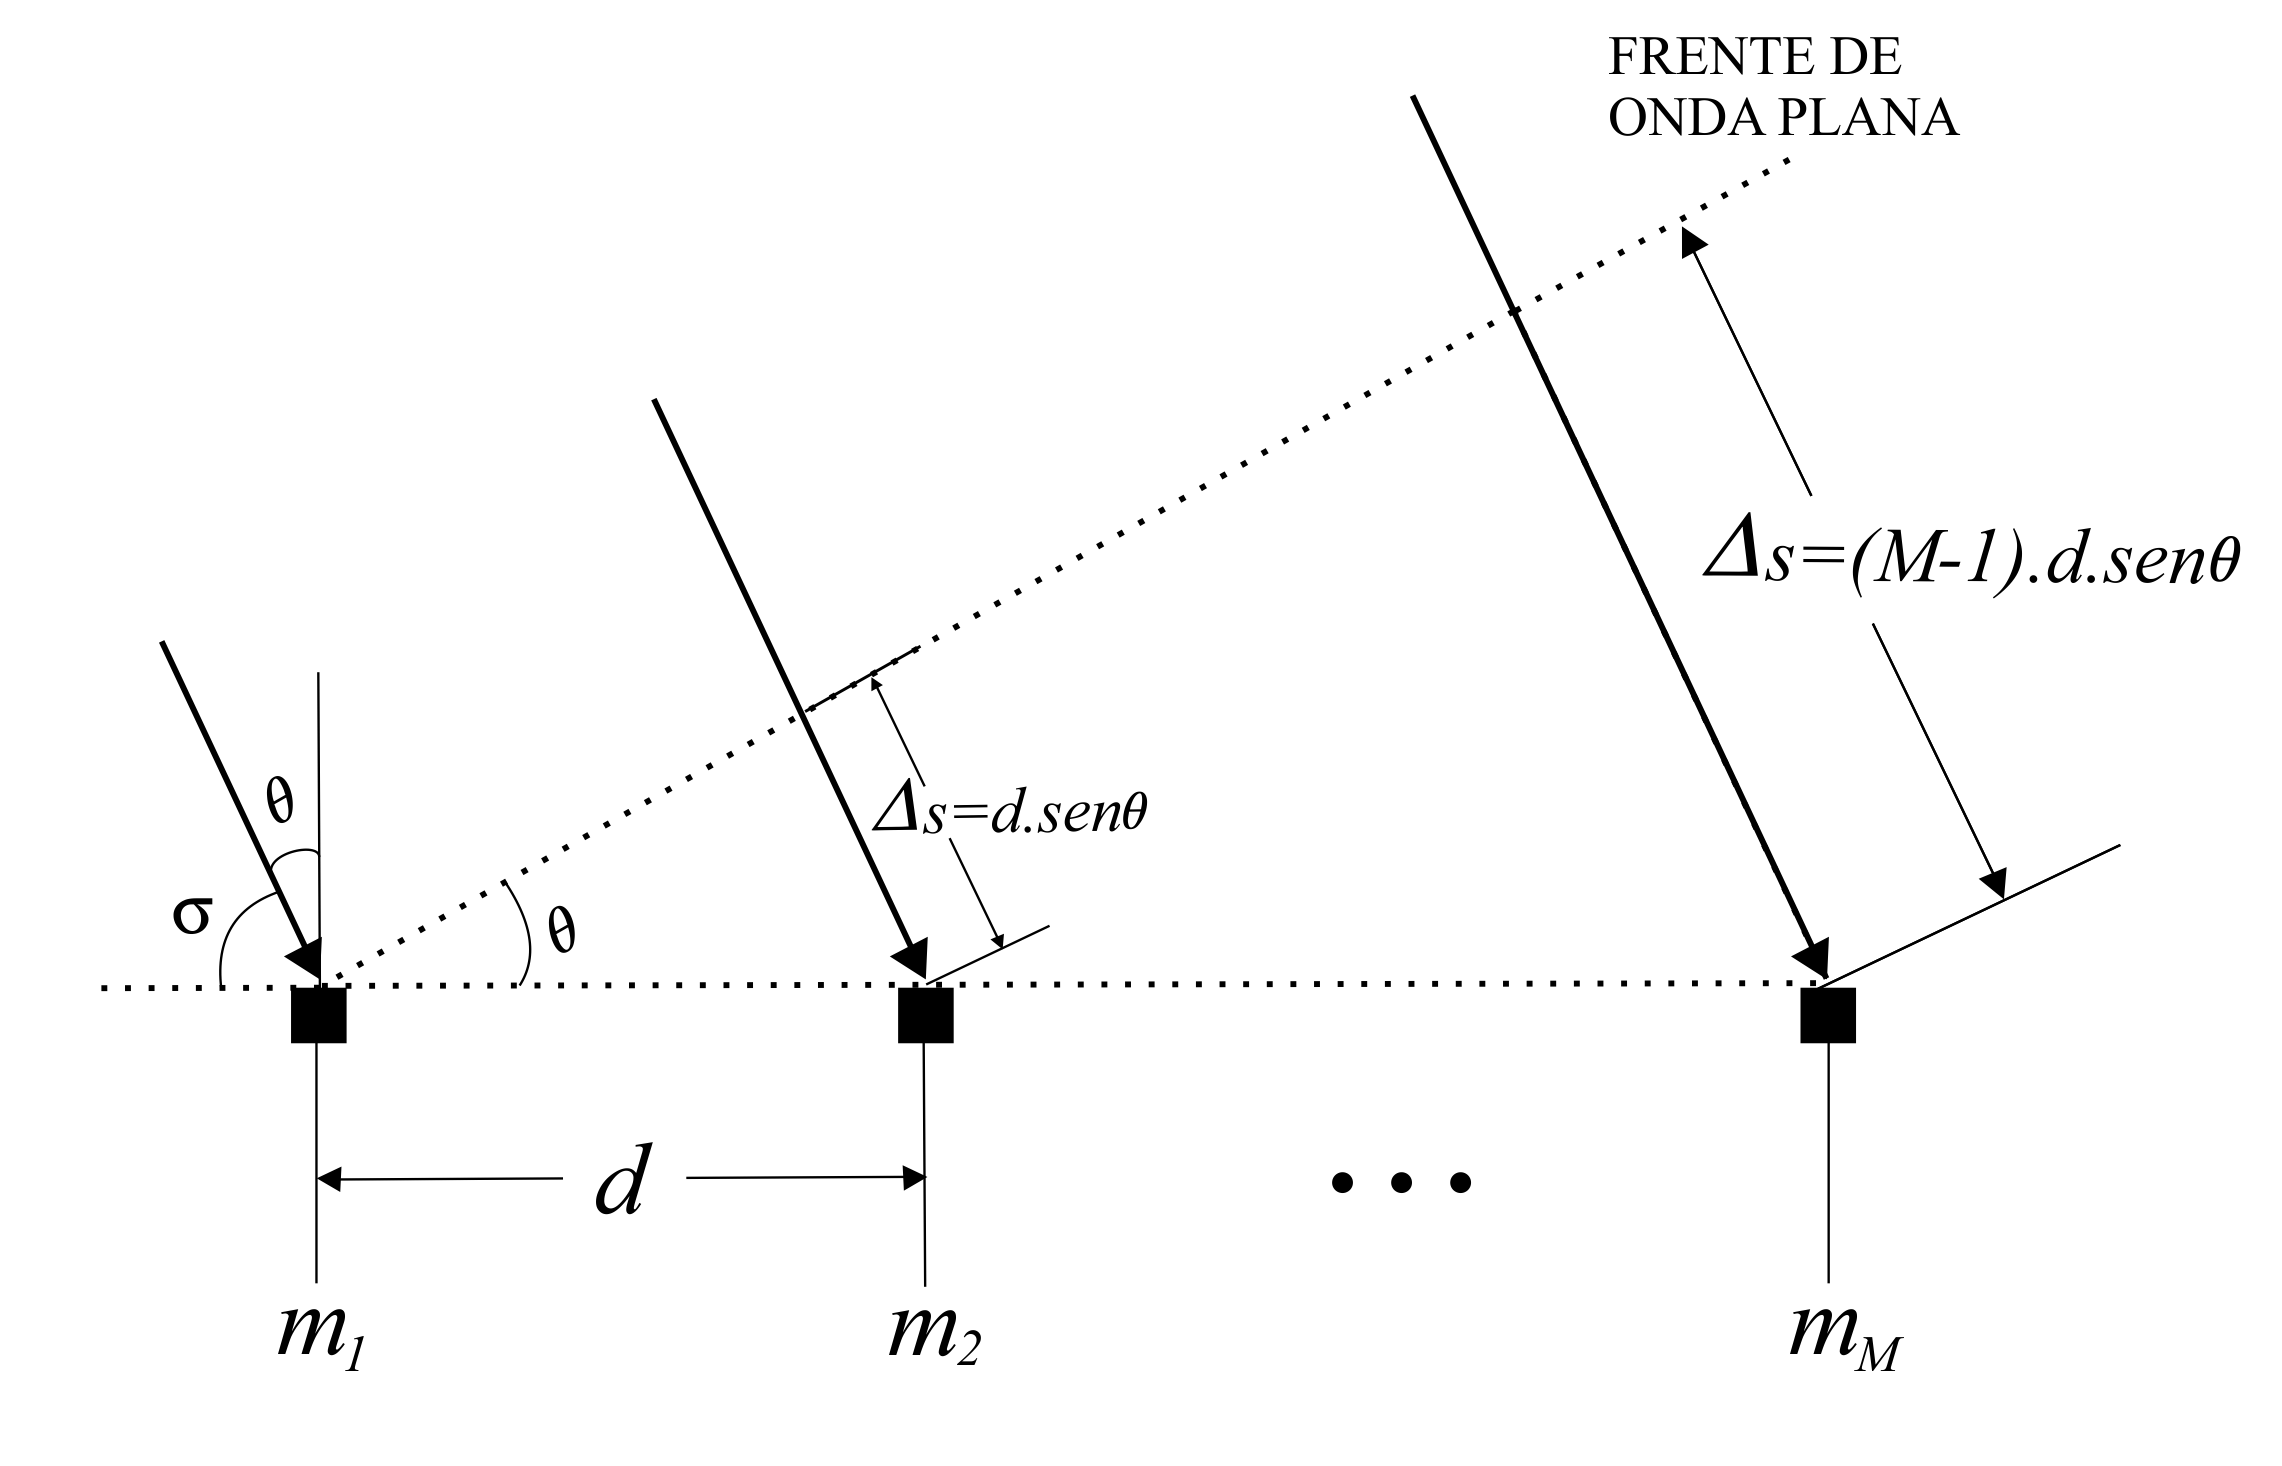
\includegraphics[width=\columnwidth]{images/DOA.png}
    \caption{Chegada da onda acústica no arranjo de microfones.}
    \label{fig:array}
\end{figure}

O atraso de tempo que a onda leva para percorrer a distância $\Delta s$, indicada na Fig.~\ref{fig:array}, é dado pela equação (\ref{eq:atraso_tempo}):
 
 \begin{equation}\label{eq:atraso_tempo}
\Delta t = \frac{d\cdot sen(\theta)}{\mu},
\end{equation}

\noindent em que $d$ é a distância entre cada microfone subsequente, e $\theta$ é o ângulo de chegada, ambos ilustrados na Fig.~\ref{fig:array}. A velocidade de propagação do som no ar ($\mu$) é aproximadamente conhecida e considerada constante. Dessa maneira é possível obter o atraso do sinal em segundos. Para obter o atraso do sinal em radiano, multiplica-se os dois lados da equação pela frequência angular ($\omega$) e tem-se:
 
\begin{equation}
\label{eq_tau}
\tau = \Delta t \cdot \omega = \frac{d\cdot sen(\theta) \cdot \omega}{\mu},
\end{equation}
 
\noindent em que $\tau$ é o atraso de chegada do sinal em radianos, e $\omega$~é~a frequência angular obtida a partir de estimação espectral (seleção da frequência dominante).

%%%%%%%%%%%%%%%%%%%%%%%%%%%%%%%%%%%%%%%%%%%%%%%%%%%%%%%%%%%%%%%%%%%%%
%%%%%%%%%%%%%%% ESTIMADOR NÃO PARAMÉTRICOS CLÁSSICOS %%%%%%%%%%%%%%%%
%%%%%%%%%%%%%%%%%%%%%%%%%%%%%%%%%%%%%%%%%%%%%%%%%%%%%%%%%%%%%%%%%%%%%

\section{ESTIMADOR NÃO PARAMÉTRICO CLÁSSICO}
\label{sec_est_classico}
A técnica de estimação de DOA usada neste artigo utiliza o periodograma para estimar a densidade espectral de potência dos sinais de cada microfone. Em seguida, a seleção de frequência dominante é realizada tomando-se o valor máximo do periodograma. A frequência dominante pode ser mapeado em fase por meio do espectro de fase do sinal. Finalmente, é possível calcular as diferenças de fases. Esta técnica destaca-se pela simplicidade, sendo uma boa candidata para sinais determinísticos, como o tom de 1~kHz utilizado neste trabalho.

O algoritmo para a estimação do atraso $\tau$ e, consequentemente, do ângulo de chegada, é ilustrado no diagrama de blocos da Fig.~\ref{fig:diagram}. O sinal atinge os microfones e é adquirido pelo ADC. No bloco seguinte é estimado o espectro com o uso do Periodograma e a seleção de frequência dominante, então, obtida a diferença de fase. Realiza-se o procedimento para os demais microfones e assim obtém-se as diferenças de fase, em relação ao primeiro microfone, utilizadas para o cálculo do ângulo de chegada. 
 
\begin{figure}[!htb]
     \centering
     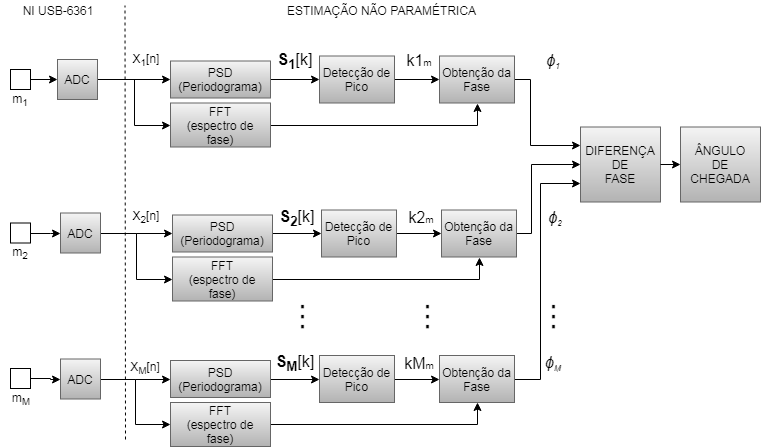
\includegraphics[width=\columnwidth]{images/angle_estimation_diagram}
     \caption{Diagrama de blocos do método de estimação de DOA.}
     \label{fig:diagram}
\end{figure}
    
 
\subsection{Periodograma}

Entre outras informações, o periodograma pode ser utilizado para identificar as frequências significativas de um sinal em termos de potência~\cite{Jenkins1961GeneralSpectra,Processes2007SpectralPeriodogram}. Neste artigo, o objetivo é encontrar a frequência do sinal emitido pela fonte (um tom de 1~kHz). 

O periodograma é obtido pela autocorrelação janelada do sinal, como mostrado na equação~(\ref{eq:autocorrelacao}):

\begin{equation}\label{eq:autocorrelacao} 
	\mathbold r[k]={\frac{1}{L}} \cdot \sum_{n=0}^{L-1} \mathbold x[n]\cdot \mathbold x[n+k]\cdot \mathbold w[n] \cdot \mathbold w[n+k]
\end{equation}

\noindent em que x[n] é o sinal recebido no sensor, e $\mathbold w[n]$ é uma janela usada para redução da variância do estimador. Neste trabalho, foi usado uma janela retangular. 

Finalmente, a PSD pode ser estimada pela transformada de Fourier da autocorrelação, como:
\begin{equation}
\mathbold {S}[k]= {\frac{1}{L}} \cdot \left|\sum_{k}^{L-1} \mathbold{r}[{k}] \cdot e^{-j\cdot \frac{2\pi kn}{L} } \right|^2.
\end{equation}

%, dada por:
%
%\begin{equation}\label{eq:janela}
%\sum_{n=1}^{L-1} \mathbold{w}[n] = 1.
%\end{equation}
	%
	%reduzir a variância dos estimadores é de incluir janelas (windows) de observação
	
	
	
 %Utilizado para calcular harmônicos e notar certos padrões presentes no sinal \cite{Jenkins1961GeneralSpectra}-\cite{Processes2007SpectralPeriodogram}, em que neste artigo o padrão a ser encontrado é um tom, por exemplo de 1 kHz, utilizado nas simulações. 
 
%No periodograma faz-se a autocorrelação do sinal que é o somatório do produto entre o sinal original e o mesmo atrasado. Obtém-se uma série de valores pelo tempo $\left\{x(0), x(1), ... x(L-1) \right\} $, em que L é o tamanho do vetor autocorrelação. No artigo utiliza-se a janela retangular na estimação espectral, representada nas equações \ref{eq:autocorrelacao} e \ref{eq:janela} por $w[n]$. Com isso a autocorrelação, do sinal $x[n]$, pode ser estimada por:





%Calculando-se a correlação cruzada tem-se o periodograma.


\subsection{Seleção de Frequência Dominante}
%Para obter a Densidade Espectral (\emph{Power Spectral Density}, PSD) do sinal, foi utilizado o Periodograma, explicado anteriormente. 

A partir da PSD estimada, como descrito na seção anterior, pode ser realizada a seleção da frequência dominante de acordo com a equação (\ref{eq:argmax}):  
 
 \begin{equation}\label{eq:argmax}
 k_m = \underset{k}{\operatorname{arg \ max}}(\mathbold {S}[k]), 
 \end{equation}

em que 

\begin{equation}
\omega = \frac{2\pi k_m}{L}.
\end{equation}


Conhecendo a frequência dominante do sinal, pode-se consultar espectro de fase do sinal, e obter a fase ($\phi_n$) correspondente ao microfone $n$~\cite{Telgarsky2013DominantExtraction}.
 
\subsection{Estimação do Ângulo de Chegada}
Realizando os passos apresentados até o momento, é possível estimar a fase de cada microfone do arranjo. Como ilustrado na Fig.~\ref{fig:delay}, a diferença de fase $\tau_{n}$ de cada microfone em relação ao primeiro pode ser calculada como:

\begin{equation}\label{eq:media_tau}
\tau_{n} = \phi_n - \phi_1.
\end{equation}

\begin{figure}[!htb]
     \centering
     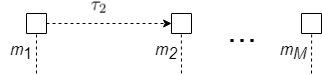
\includegraphics[scale=0.4]{images/delay_microphones.png}
     \caption{Atraso entre microfones.}
     \label{fig:delay}
\end{figure}

Para obter um valor mais preciso da diferença de fase, calcula-se um $\tau$ relacionado com todos os microfones, como a seguir:
\begin{equation}\label{eq:media_tau}
\tau = \frac{1}{M-1}\sum_{n=2}^{M} \frac{\tau_n}{n-1}.
\end{equation}


Para obter a estimação do ângulo de chegada do sinal, isola-se $\theta$ da Equação~(\ref{eq_tau}), resultando em:
\begin{equation}
\sigma = 90-\arcsin \left(\frac{\tau \cdot \mu}{d \cdot \omega} \right ),
\end{equation} 
 
\noindent em que $\sigma$ é o ângulo de chegada do sinal em relação ao eixo do arranjo de microfones, como ilustrado na Fig.~\ref{fig:array}.
 
%%%%%%%%%%%%%%%%%%%%%%%%%%%%%%%%%%%%%%%%%%%%%%%%%%%%%%%%%%%%%%%%%%%%%
%%%%%%%%%%%%%%% GERAÇÃO DE SINAIS E SETUP DE MEDIÇÃO %%%%%%%%%%%%%%%%
%%%%%%%%%%%%%%%%%%%%%%%%%%%%%%%%%%%%%%%%%%%%%%%%%%%%%%%%%%%%%%%%%%%%%

\section{SINAIS SIMULADOS E SETUP DE MEDIÇÃO}
\label{sec_gera_sinal}
O estimador discutido na seção anterior foi implementado em software, validado com sinais sintéticos e testado em um sinal acústico real adquirido com um \textit{setup} de medição próprio, mostrado na Fig.~\ref{fig:setup}.  
\begin{figure}[!htb]
    \centering
    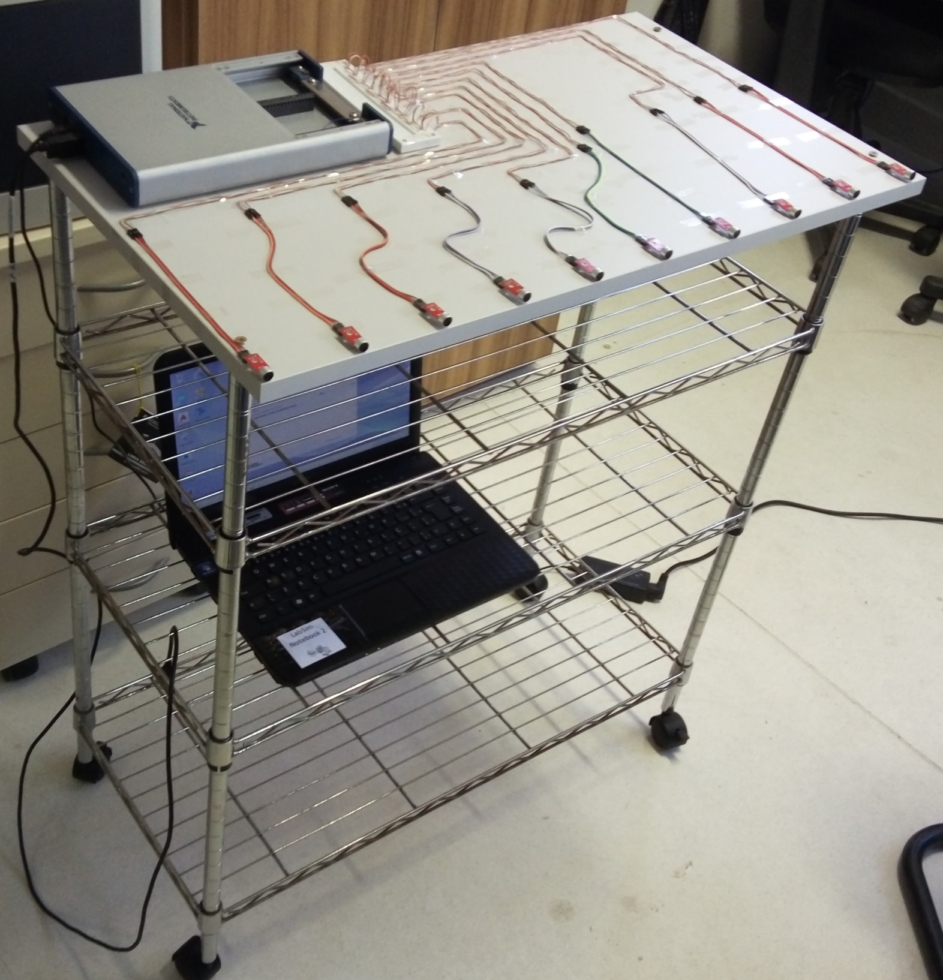
\includegraphics[width=\columnwidth]{images/setup.jpg}
    \caption{\textit{Setup} de aquisição de sinais.}
    \label{fig:setup}
\end{figure}

\subsection{Geração de sinais sintéticos} 
Um passo importante antes de realizar experimentos reais é a análise em ambiente simulado. Com os sinais sintéticos gerados no simulador, foi realizada uma análise do método proposto variando a Relação Sinal-Ruído (\emph{Signal-to-Noise Ratio}, SNR) do sinal recebido. O sinal sintético foi modelado como na Equação~(\ref{eq:sinalruido}):

\begin{equation}\label{eq:sinalruido}
\mathbold{y}(t) = \mathbold{A}(\phi) \mathbold{S}(t) + \mathbold{N}(t),
\end{equation}

\noindent em que $\mathbold{S}(t)$ é o sinal emitido pela fonte, $\mathbold{N}(t)$ é o ruído adicionado ao sinal e $\mathbold{A}(\phi)$ representa o vetor de atraso dos microfones, escrito como nas Equações~(\ref{eq:atrasos}) e (\ref{eq:atrasos2}):

\begin{equation}\label{eq:atrasos}
\mathbold{A}(\phi) = [\mathbold{a}(\phi_1), \mathbold{a}(\phi_2), \dots , \mathbold{a}(\phi_n)]
\end{equation}

\begin{equation}
\label{eq:atrasos2}
\mathbold{a}(\phi_n) = [1, e^{j \omega }, \dots , e^{j \omega (M-1)}]^T
\end{equation}

% \begin{equation}\label{eq:atrasos}
% \bf{A}(\phi) = [\bf{a}(\it{\phi_1}), a(\it{\phi_2}), \dots , a(\it{\phi_n})] 
% \end{equation}

%Em que $\mathbf{y}$ é o sinal modelado e, o $\mathbf{N}$ é o ruído adicionado.
%Em que \bf{y(\it{t})}  é o sinal modelado e, o \bf{N(\it{t})}  é o ruído adicionado.
\subsection{Medição de sinais reais}
O \textit{setup} de medição (Fig.~\ref{fig:setup}) foi composto dos seguintes equipamentos:
\begin{itemize}
	\item Um aquisitor NI USB-$6361$ da National Instruments;
	\item Dez microfones FC-$109$;
	\item Um notebook Sony Vaio PCG-61A11X;
	\item Uma caixa de som JBL Flip $3$.
\end{itemize}

Em uma mesa de $90$ cm de altura,  os $10$ microfones foram organizados como um Arranjo Linear Uniforme (ULA), espaçados a uma distância $d=8$~cm. Com a mesa parada em uma determinada posição, cada bateria de medição consistiu em posicionar a fonte sonora (Caixa JBL Flip $3$) a uma distância predeterminada do primeiro microfone, com também $90$~cm de altura em relação ao solo. A distância predeterminada entre a fonte e a mesa de medição respeita a definição de campo distante e estabelece uma linha de visada direta entre elas. O experimento realizado assumiu que a distância do primeiro microfone para a única fonte foi de 8~m, com ângulo de $30\degree$. A medições foram realizadas em ambiente silencioso, evitando interferência cocanal, e possibilitando emular a presença somente de ruído.

  
%Ao verificar o método nas simulações realizadas, o próximo passo consistiu em realizar o experimento para dados reais com setup de medição próprio. No setup, para aquisição de dados, utilizou-se um aquisitor NI USB-$6361$ da National Instruments, microfones FC-$109$, notebook Sony Vaio PCG-61A11X e uma caixa de som JBL Flip $3$, em que foram realizados diversas aquisições em ambiente real para um teste consistente do método proposto.
 
%Em uma mesa de $90$ cm de altura foram alocados $10$ microfones organizados como um Arranjo Linear Uniforme (ULA-\textit{Uniform Linear Array}), espaçados a uma distância $d =8$ cm. Com o setup fixado em uma determinada posição, cada bateria de medição consistiu em posicionar a fonte sonora (Caixa JBL Flip $3$) a uma distância X do primeiro microfone, com $90$ cm de altura em relação ao solo. Em que X respeita a definição de campo distante e entre os objetos há uma linha de visada direta. 



Como descrito na Seção~\ref{sec_rel_works}, as medições foram realizadas em um local representativo do uso do arranjo de microfones para aplicações em ambientes universitários e condomínios residenciais, bem similar ao cenário \emph{Dual-stripe} definido pelo 3GPP~\cite{3GPP_R4_092042}. 
  

\section{RESULTADOS}
\label{sec_res}

Para construção das curvas de desempenho envolvendo os sinais sintéticos utilizou-se janelas de 400 amostras do sinal para construir o periodograma e estimar o ângulo. Assim, para melhor visualização das curvas, a janela foi deslocada 10000 vezes, gerando 10000 experimentos independentes de recepção do sinal e estimação do ângulo. Para os sinais medidos, a janela foi de 4000 amostras.

\subsection{Validação com sinais sintéticos}

A Fig.~\ref{fig:PSD} mostra o periodograma com janela retangular para três sinais sintéticos sujeitos a SNR igual à 0, 5 e 15~dB. A principal observação é sobre o desempenho satisfatório do periodograma na estimação do pico espectral, resultando na convergência do pico espectral para a frequência de 1~kHz para os três valores de SNR analisados. Esses gráficos são resultado da média dos periodogramas dos dez microfones do arranjo.
%A estimação do espectro utilizando periodograma com a janela retangular teve um desempenho satisfatório, tendo o máximo de todos os microfones definido de forma convincente, como mostra a Fig.~\ref{fig:PSD}, em que os picos dos microfones convergem para uma mesma frequência.
\begin{figure}[!htb]
     \centering
     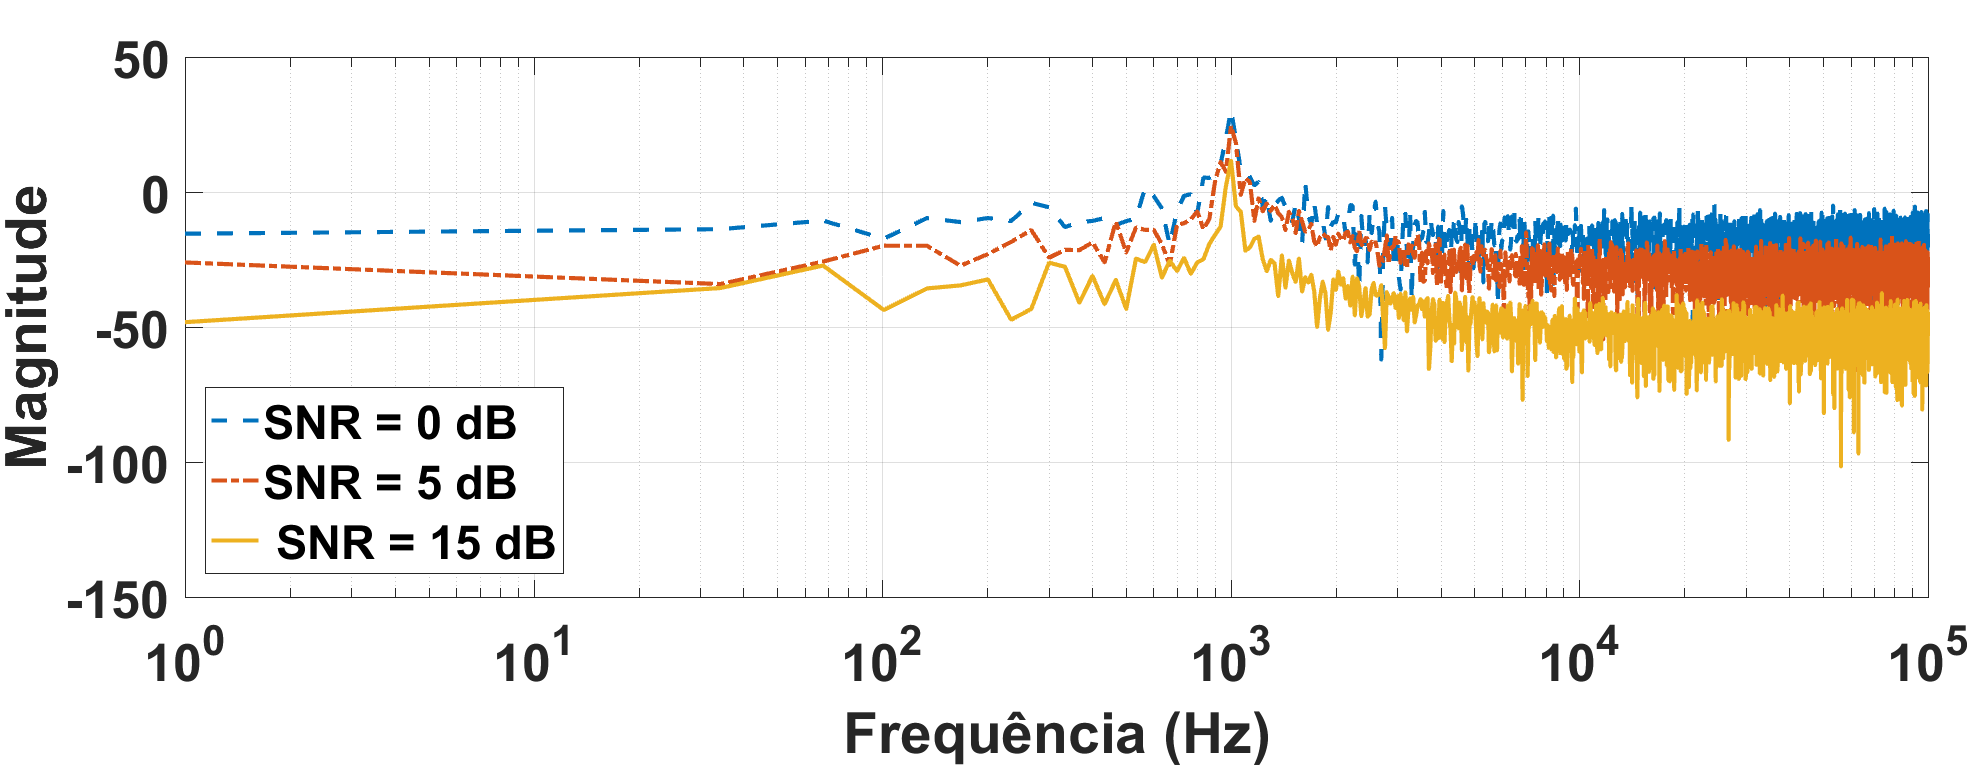
\includegraphics[width=\linewidth]{images/PSD_simulation}
     \caption{Periodograma para dados sintéticos para SNR igual à 0, 5 e 15.}
     \label{fig:PSD}
\end{figure}

Outra abordagem para validação dos dados sintéticos foi realizar o cálculo do Erro Médio Quadrático (\emph{Mean Squared Error}, MSE) entre o ângulo conhecido (usado para gerar o sinal da fonte) e o ângulo estimado. Para tal fim, a Fig.~\ref{fig:rmse_snr} mostra o MSE para alguns valores de SNR. Observando a figura, visualiza-se a diminuição do MSE ao passo que a SNR cresce, mostrando uma consistência qualitativa tanto na geração do sinal sintético quanto na implementação do periodograma.

%Para uma melhor visualização dessa análise, foi plotado o MSE em função da Relação Sinal-Ruído (\emph{Signal-to-Noise Ratio}, SNR), mostrado na Fig.~\ref{fig:rmse_snr}, em que visualiza-se a diminuição do MSE ao passo que a SNR cresce, mostrando uma consistência.

\begin{figure}[!htb]
     \centering
     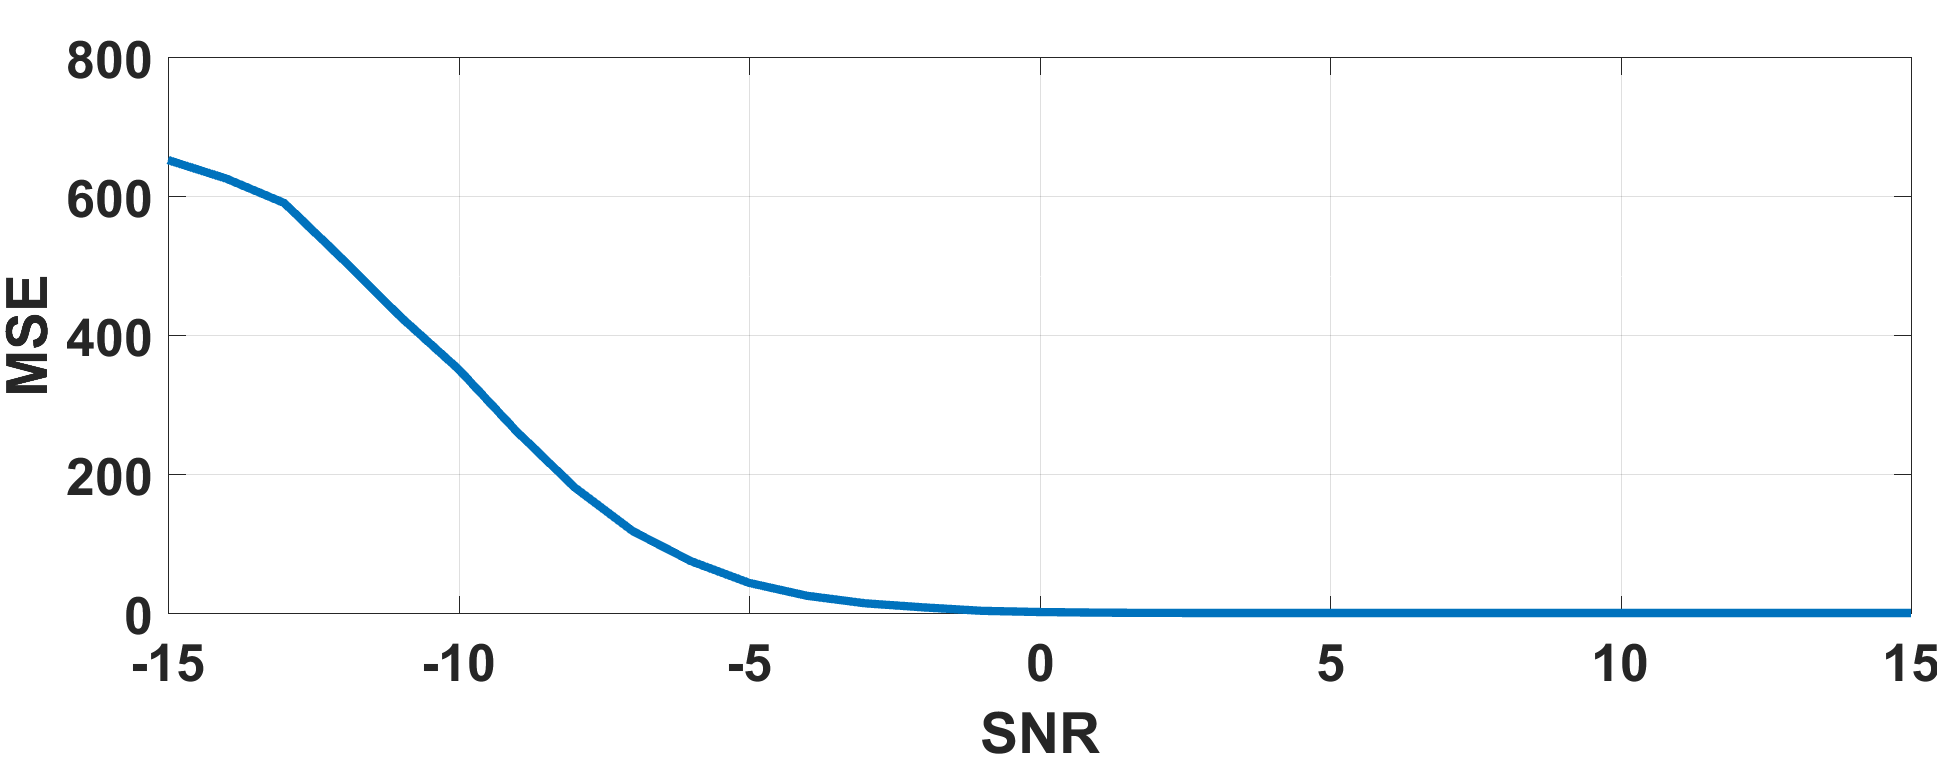
\includegraphics[width=\linewidth]{images/emq_vs_snr}
     \caption{MSE do ângulo com a variação da SNR (sinal sintético).}
     \label{fig:rmse_snr}
\end{figure}

Finalmente, objetivando analisar a confiabilidade na estimação do ângulo, a Fig.~\ref{fig:var_snr} mostra a variância dos ângulos estimados nos 10000 experimentos envolvendo o sinal sintético. Mais uma vez se observou consistência com o decaimento da variância ao passo do crescimento da SNR.


%para os mesmos dados citados (ângulos conhecidos e e ângulos encontrados). A Fig.~\ref{fig:var_snr} ilustra o comportamento da variância entre os dados em função da SNR, mostrando consistência ao decair ao passo do crescimento da SNR.

\begin{figure}[!htb]
     \centering
     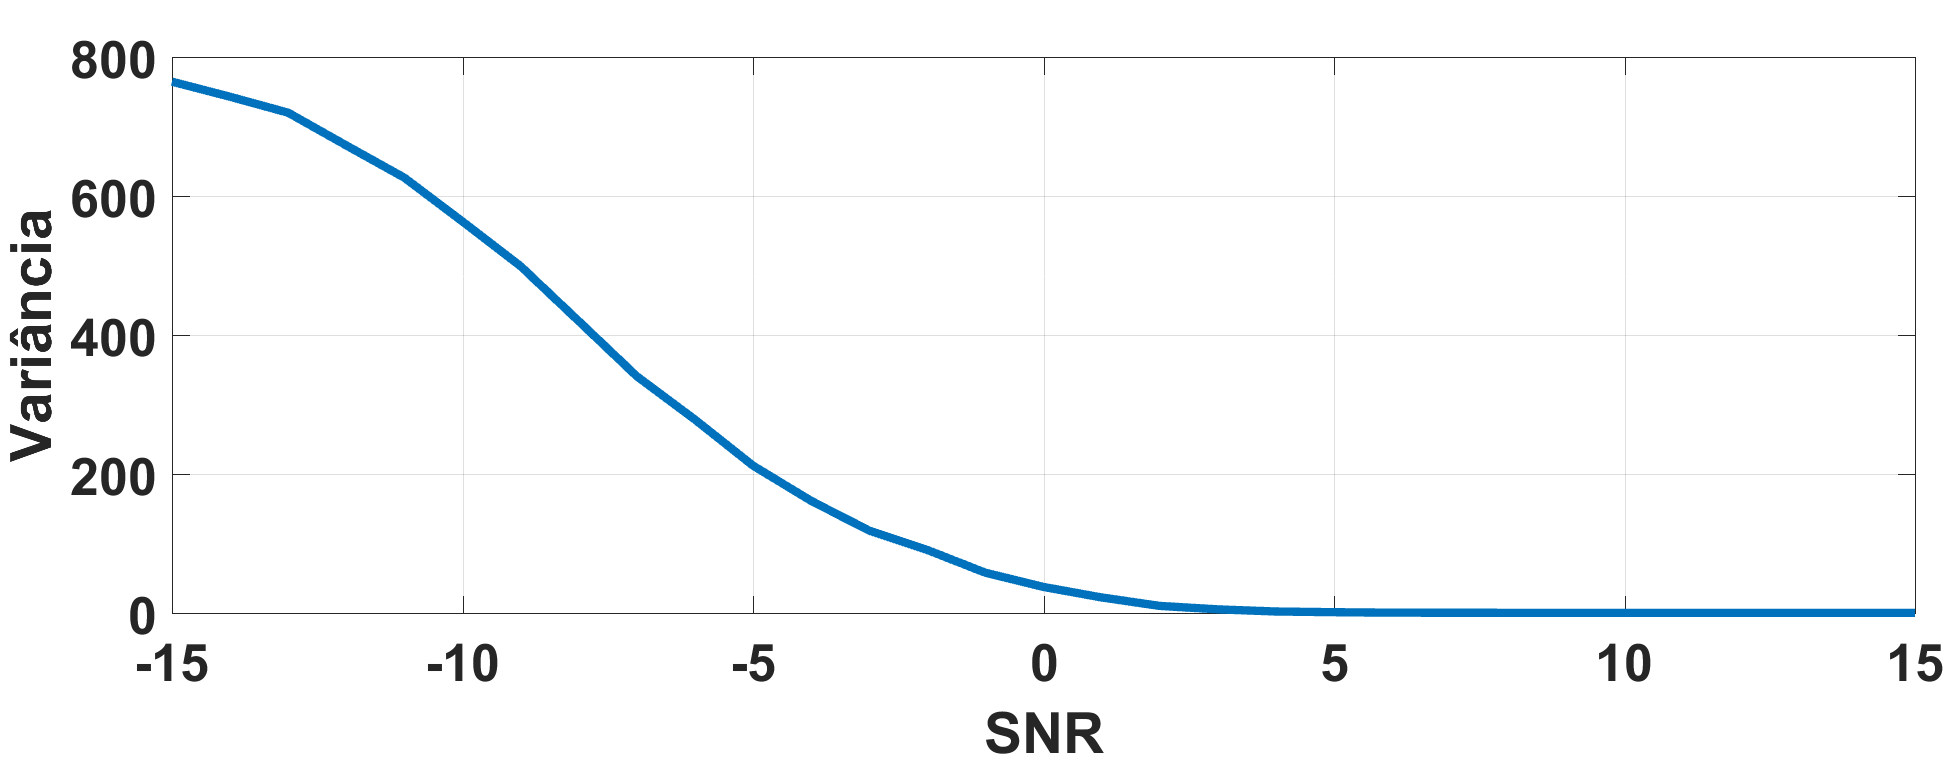
\includegraphics[width=\linewidth]{images/var_vs_snr}
     \caption{Variância dos ângulos estimados (sinal sintético).}
     \label{fig:var_snr}
\end{figure}

Considerando que o periodograma é um estimador simples e de baixo custo computacional, os resultados da simulação foram os esperados, obtendo um desempenho insatisfatório para SNRs baixas e resultados consistentes para SNRs altas.  
 
\subsection{Resultados Experimentais}
A Fig.~\ref{fig:PSD_real} mostra o resultado do periodograma médio considerando todos os microfones. É possível visualizar a coerência dos resultados dos diversos microfones, que convergem para uma mesma frequência, mesmo quando o método de estimação é simples, como o periodograma.
%Com os dados reais, utilizando o Periodograma, foram analisados snapshots de $4000$ amostras do sinal e plotada a PSD de cada microfone do arranjo, tornando possível visualizar a coerência entre os microfones que convergem para uma mesma frequência, como ilustrado no gráfico da Fig.~\ref{fig:PSD_real}, que mostra a PSD feita a partir da média dos dados de cada microfone.
\begin{figure}[!htb]
     \begin{center}
     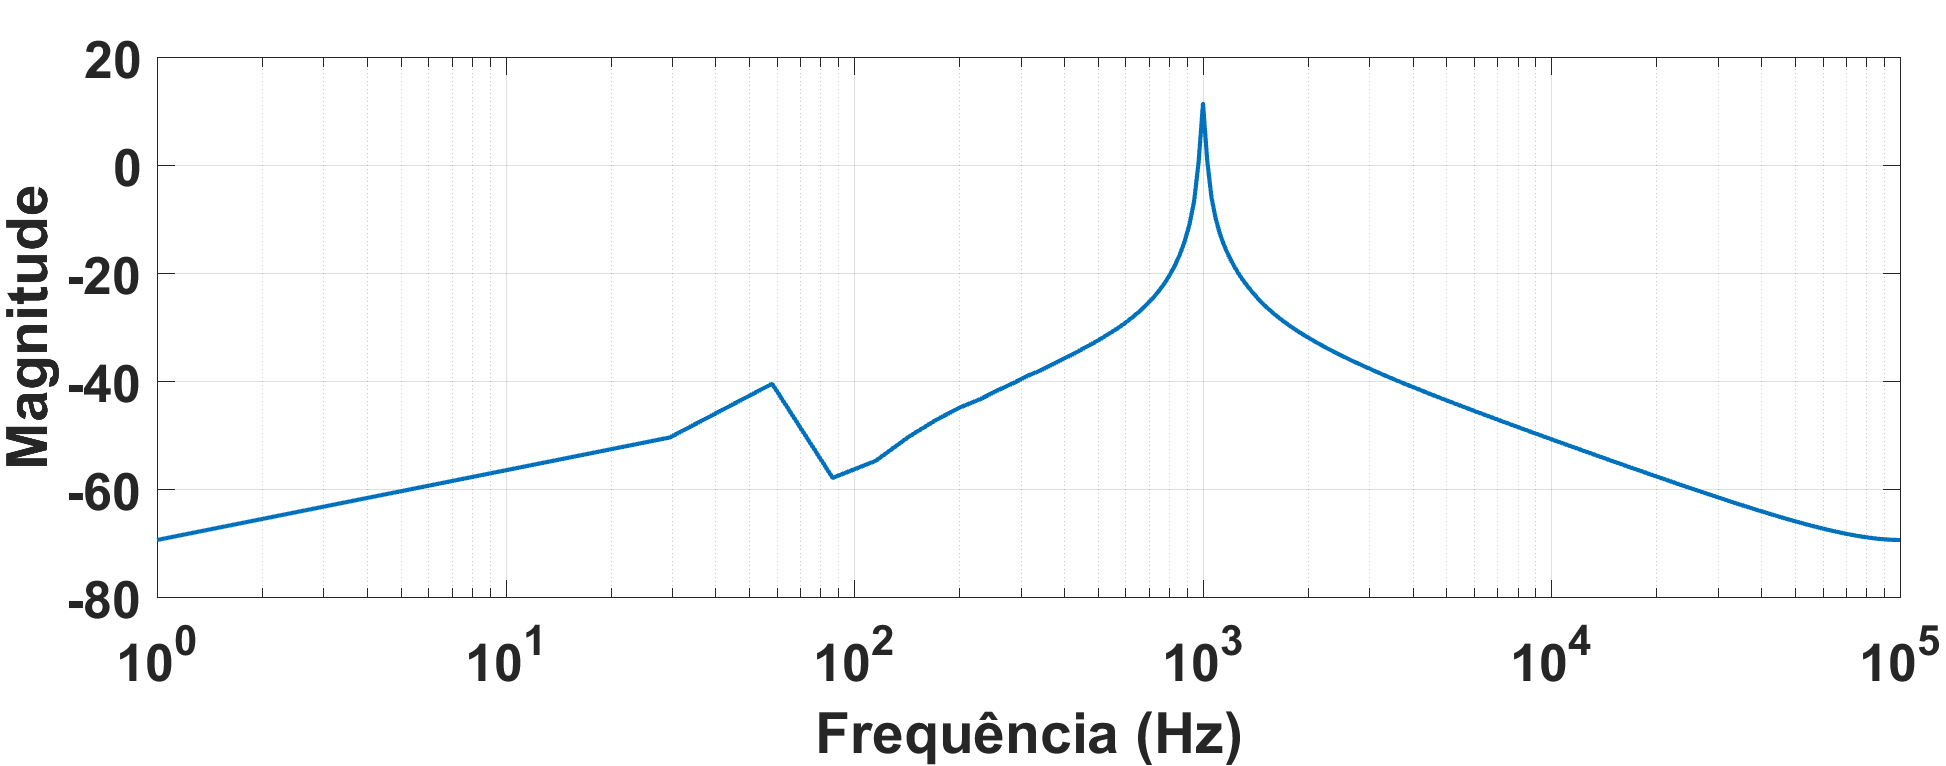
\includegraphics[width=\linewidth]{images/PSD_data_real}
     \end{center}
     \caption{Periodograma para dados reais.}
     \label{fig:PSD_real}
\end{figure}

De posse do espectro de fase do sinal e com estimação da frequência obtida pelo periodograma, a estimação do ângulo de chegada foi realizada e comparada com o ângulo da fonte ($30\degree$). O ângulo estimado foi de $31,6\degree$ (média de todos os experimentos), mostrando a eficácia do método para os dados reais, pelo baixo MSE (2,81).

%%%%%%%%%%%%%%%%%%%%%%%%%%%%%%%%%%%%%%%%%%%%%%%%%%%%%%%%%%%%%%%%%%%%%
%%%%%%%%%%%%%%%% CONCLUSÕES E TRABALHOS FUTUROS %%%%%%%%%%%%%%%%%%%%%
%%%%%%%%%%%%%%%%%%%%%%%%%%%%%%%%%%%%%%%%%%%%%%%%%%%%%%%%%%%%%%%%%%%%%

\section{CONCLUSÕES E TRABALHOS FUTUROS}
\label{sec_conclu}

Com as comparações realizadas, percebe-se que o periodograma utilizando janela retangular obteve um desempenho satisfatório para estimação da densidade espectral de potência para SNRs altas, possibilitando uma boa estimação de ângulo, e, como esperado, um resultado adverso para SNRs severas, afetando a precisão da estimação. Esse método pode ser uma boa escolha para validação de \textit{setups} de medição, configurando o sinal da fonte em ângulos predefinidos e verificando, em situação de alta SNR, se o \textit{setup} de aquisição não está causando desvios significativos na estimação de ângulo do periodograma.

A continuação deste trabalho considera o estudo de diferentes tipos de janelas aplicadas ao periodograma e a análise do impacto de cada uma na detecção de ângulo de chegada. Outro caminho de investigação é a aplicação de outros método de estimação em cenários mais desafiadores, como os que envolve interferência cocanal.

%\section{AGRADECIMENTOS}

%Os autores gostariam de agradecer a Roger Brendo Almeida de Medeiros pela contribuição na elaboração das figuras.

%%%%%%%%%%%%%%%%%%%%%%%%%%%%%%%%%%%%%%%%%%%%%%%%%%%%%%%%%%%%%%%%%%%%%
%%%%%%%%%%%%%%%%%%%%%%%%%% BIBLIOGRAFIA %%%%%%%%%%%%%%%%%%%%%%%%%%%%%
%%%%%%%%%%%%%%%%%%%%%%%%%%%%%%%%%%%%%%%%%%%%%%%%%%%%%%%%%%%%%%%%%%%%%

%\bibliographystyle{ieeetr}
\bibliographystyle{IEEEtran}
\bibliography{Mendeley_DOA_nonparametric}

% \begin{thebibliography}{99}

% \bibitem{c3}Noise Robust Direction of Arrival Estimation for Speech Source With Weighted Bispectrum Spatial Correlation Matrix
% \end{thebibliography}


\end{document}
